\documentclass[conference]{IEEEtran}

\usepackage[noadjust]{cite}

\usepackage[dvips]{graphicx}

\usepackage{url}
\usepackage[cmex10]{amsmath}
\interdisplaylinepenalty=2500
\usepackage{threeparttable}
\usepackage{multirow}

\begin{document}

\title{Using Altruistic Peers to Help With Free Web Downloads}
\author{\IEEEauthorblockN{Cameron Dale}
\IEEEauthorblockA{School of Computing Science\\
Simon Fraser University\\
Burnaby, British Columbia, Canada\\
Email: camerond@cs.sfu.ca}}

\maketitle

\begin{abstract}
A large amount of free content is available over the Internet from
many different distributors. Most of this content uses the traditional
client-server model to handle requests from users. However, there is an
opportunity to use peer-to-peer techniques to reduce the cost of
much of this distribution, especially due to the altruistic nature
of many of these users. We present a general technique for
satisfying the needs of this P2P distribution, which is applicable
to many of these distributors systems. Our method makes use of a DHT
for storing the location of peers, using the cryptographic hash of
the file as a key. We then go further and implement a solution for
the distribution of Debian software packages.
\end{abstract}

%%%%%%%%%%%%%%%%%%%%%%%%%%%  Section  %%%%%%%%%%%%%%%%%%%%%%%%%%%%

\section{Introduction}
\label{intro}

There are a large number of free content distributors using
package distribution systems over the Internet to distribute content
to their users. These distributors have developed many different
methods for this distribution, but they almost exclusively use a client-server
model to satisfy user requests. The popularity and number of users
results in a large number of requests, which usually requires a
network of mirrors to handle. Due to the free nature of this
content, many users are willing and able to contribute upload
bandwidth to this distribution, but have no current way to do this.

We present a new peer-to-peer distribution model to meet these
demands. It is based on many previous implementations of successful
peer-to-peer protocols, especially distributed hash tables (DHT) and
BitTorrent. The model relies on the pre-existence of cryptographic
hashes of the content, which should uniquely identify it for a
request from other peers. If the peer-to-peer download fails, then
the original request to the server is used as a fallback to prevent
any dissatisfaction from users. The peer can then share this new
content with others through the P2P system.

First, we examine the opportunity that is available for many of
these free content distributors. We present an overview of a system
that would efficiently satisfy the demands of a large number of
users, and should significantly reduce the currently substantial
bandwidth requirements of hosting this content. We then present an
example implementation based on the Debian package distribution
system. This implementation will be used by a large number of users,
and serves as an example for other free content distributors of the
opportunity that can be met with such a system.

%%%%%%%%%%%%%%%%%%%%%%%%%%%  Section  %%%%%%%%%%%%%%%%%%%%%%%%%%%%

\section{Related Work}
\label{related}

There are many peer-to-peer implementations available today, but
none is very well suited to this specific problem.

Many distributors make their content available in some form using
BitTorrent \cite{COHEN03}, e.g. for the distribution of CD
images. This is not an ideal situation though, as it requires the
peers to download large amounts of content that they are not
interested in, and prevents them from updating to new content
without downloading another image containing a lot of the same
content they already have. There have also been other attempted
implementations, usually based on some form of BitTorrent, to
address this problem. Unfortunately, BitTorrent is not ideally
suited to an application such as this one, for the following
reasons:
\begin{itemize}
 \item The packages are too small and there are too many to create
       individual torrents for each one.
 \item All the packages together are too large to track efficiently
       as a single torrent.
 \item BitTorrent's piece sizes are bigger than many of the
       packages, which wastes bandwidth downloading parts of other
       packages.
 \item A small number of the packages can be updated every day,
       requiring a new torrent and splitting the
       download population (even though peers in the new torrent
       share 99\% of the files in common with peers in the old
       torrent).
 \item Incentives to share (upload) are no longer needed, as the
       content is freely available for anyone to download without
       sharing (seeds are also not needed).
\end{itemize}

Some other implementations have used BitTorrent almost unmodified,
while others have only looked at using DHTs to replace the tracker
in a BitTorrent system. apt-torrent \cite{apttorrent} creates
torrents for some of the larger content available, but it ignores
the smaller content, which is often the most popular.
DebTorrent \cite{debtorrent} makes widespread modifications to a
traditional BitTorrent client, but also requires some changes to the
distribution system to support it, and separates peers into groups
based on their interest which limits the effectiveness of the
sharing. Kenosis \cite{kenosis} is a P2P Remote Procedure Call
client also based on the Kademlia DHT, but it is meant as a P2P
primitive system on which other tools can be built, and so it has no
file sharing functionality at all. Many have used a DHT as a drop-in
replacement for the tracker in a BitTorrent system
\cite{bittorrent-dht, azureus-dht}, but such systems only use the
DHT to find peers for the same torrent, so the file sharing uses
traditional BitTorrent and so is not ideal for the reasons listed
above.

%%%%%%%%%%%%%%%%%%%%%%%%%%%  Section  %%%%%%%%%%%%%%%%%%%%%%%%%%%%

\section{Situation}
\label{situation}

There are a large number of groups using the Internet to distribute
their free content. This content is usually available from a free
download site, which usually requires a network of mirrors to
support the large number of requests. This content almost always
supports some kind of file verification, usually cryptographic
hashes, to verify the completed downloads accuracy or authenticity.

\subsection{Examples}
\label{examples}

Most Linux distributions use a software package management system
that fetches packages to be installed from a network of mirrors. The
Debian project \cite{debian} (and other Debian-based distributions)
uses the \texttt{apt} program, which downloads Debian packages in
the \texttt{.deb} format from one of many mirrors. The program will
first download index files that contain a listing of which packages
are available, as well as important information such as their size,
location, and a hash of their content. Red Hat's Fedora project
\cite{fedora} (and other RPM-based distributions) use the
\texttt{yum} program to obtain RPMs, and Gentoo \cite{gentoo} uses
\texttt{portage} in a similar way.

Other software vendors also use a similar system. CPAN \cite{cpan}
distributes files containing software packages for the PERL
programming language, using SOAP RPC requests to find and download
files. Cygwin \cite{cygwin} provides many of the
standard Unix/Linux tools in a Windows environment, using a
package management tool that requests packages from websites. There
are two software distribution systems for Mac OSX, fink and
MacPorts, that also retrieve packages in this way.

Also, some systems use direct web downloads, but with a hash
verification file also available for download next to the desired
file. These hash files usually have the same file name, but with an
added extension identifying the hash used (e.g. \texttt{.md5} for
the MD5 hash).

Finally, there are other programs that use cryptographic hashing to
identify files. Git is a version control system in which all files,
commits, and tags, are identified by their SHA1 hash. These hashes
are used to verify the origin of these items, but are also used when
clients update their local files with new remote information.

\subsection{Similarities}
\label{similarities}

The important things to note for each of the systems mentioned in
section \ref{examples}, is that they all have the following in
common:
\begin{itemize}
 \item The content is avaliable for anyone to freely download.
 \item The content is divided into distinct units (packages), each of which contains
       a small independent part of all the content.
 \item Users are typically not interested in downloading all of the content
       available.
 \item Hashes of the content and its size are available before the
       download is attempted.
 \item Requests for the content are sent by a tool, not directly by
       the user (though the tool is responding to requests from the user).
\end{itemize}

We also expect that there are a number of users of these systems
that are motivated by altruism to want to help out with this
distribution. This is common in these systems due to the free nature
of the content being delivered, which encourages some to want to
help out in some way. A number of the systems are also used by
groups that are staffed mostly, or sometimes completely, by
volunteers. This also encourages users to want to \emph{give back}
to the volunteer community that has created the content they are
using.

\subsection{Differences}
\label{differences}

Although at first it might seem that a single all-reaching solution
is possible for this situation, there are some differences in each
system that require independent solutions. The systems all use
different tools for their distribution, so any implementation would
have to be specific to the tool it is to integrate with. In
particular, how to obtain requests from the tool or user, and how to
find a hash that corresponds to the file being requested, is very
specific to each system.

Also, there may be no benefit in creating a single large solution to
integrate all these problems. For one, though they sometimes
distribute nearly identical content (e.g. the same software
available in multiple Linux distributions), it is not exactly
identical and has usually been tailored to the system. The small
differences will change the hash of the files, and so
will make it impossible to distribute similar content
across systems. And, although peer-to-peer systems scale very well
with the number of peers in the system, there is some overhead
involved, so having a much larger system of peers would mean that
requests could take longer to complete.

%%%%%%%%%%%%%%%%%%%%%%%%%%%  Section  %%%%%%%%%%%%%%%%%%%%%%%%%%%%

\section{Opportunity}
\label{opportunity}

The situation described in section \ref{situation} presents a clear
opportunity to use some form of peer-to-peer file-sharing protocol.
This sparse interest in a large number of packages, and constant
updating, is well suited to the functionality provided by a
Distributed Hash Table (DHT). DHTs require unique keys to store and
retrieve strings of data, for which the cryptographic hashes used by
these package management systems are perfect for. The stored and
retrieved strings can then be pointers to the peers that have the
content package that hashes to that key. A downloading peer can
lookup the package hash in the DHT and, if it is found,
download the file from those peers and verify the content. If the
package hash can not be found in the DHT, the peer will fallback to
downloading from the original content location (i.e. the network of
mirrors), and once complete will add a new entry to the DHT
indicating that it has the content.

\subsection{Implementation Options}
\label{imp_options}

There are several ways to implement the desired P2P functionality
into the existing package management software. The functionality can
be directly integrated into the software, though this can be
difficult as the DHT should be running at all times, both for
efficient lookups and to support uploading of already downloaded
content, whereas the tools typically only run until the download request is complete.
Many of the package management software implementations use
HTTP requests to download the files, which makes it possible to
implement the P2P aspect as a standard HTTP caching proxy, which
will get uncached requests first from the P2P system, and then
fallback to the normal HTTP request from a server. For methods that
don't use HTTP requests, other types of proxies may also be
possible.

\subsection{Downloading From Peers}
\label{downloading}

Downloading a file efficiently from a number of peers is where
BitTorrent shines as a peer-to-peer application. Its method of
breaking up larger files into sub-pieces, each with its own hash,
makes it very easy to parallelize the downloading process and
maximize the download speed. For very small packages (i.e. less than
the sub-piece size), this parallel downloading is not necessary, or
even desirable. However, this method can still be used in
conjunction with the DHT, for the larger packages that are
available.

Since the package management system only stores a hash of the entire
content, and not of sub-pieces of that content, we will need to be
able to store and retrieve these sub-piece hashes using the P2P protocol.
In addition to storing the file download location in the DHT (which would still
be used for small files), a peer will store a \emph{torrent string}
containing the peer's hashes of the sub-pieces of the larger
files. These piece hashes could be compared ahead of time to
determine which peers have the same piece hashes (they all should),
and then used during the download to verify the downloaded pieces.

For very large files (5 or more pieces), the torrent strings
are too long to store in the DHT (a single UDP packet should be less
than 1472 bytes to avoid fragmentation). Instead, the peers will
store the torrent string for large files separately in the DHT, and
only contain a reference to it in their stored value for the hash of
the file. The reference would be a hash of the torrent string. If
the torrent string is short enough to store in the DHT (i.e. less
than 1472 bytes, or 70 pieces for the SHA1 hash), then a
lookup of that hash in the DHT would give the torrent-like string.
Otherwise, a request to the peer for the hash (using the same
method as file downloads), should return the torrent string.

% This can cause a problem with hash checking the returned data, as
% hashes for the pieces are not known. Any file that fails a hash
% check should be downloaded again, with each piece being downloaded
% from different peers than it was previously. The peers are shifted
% by 1, so that if a peers previously downloaded piece i, it now
% downloads piece i+1, and the first piece is downloaded by the
% previous downloader of the last piece, or preferably a previously
% unused peer. As each piece is downloaded the running hash of the
% file should be checked to determine the place at which the file
% differs from the previous download.
% 
% If the hash check then passes, then the peer who originally provided
% the bad piece can be assessed blame for the error. Otherwise, the
% peer who originally provided the piece is probably at fault, since
% he is now providing a later piece. This doesn't work if the
% differing piece is the first piece, in which case it is downloaded
% from a 3rd peer, with consensus revealing the misbehaving peer.

%%%%%%%%%%%%%%%%%%%%%%%%%%%  Section  %%%%%%%%%%%%%%%%%%%%%%%%%%%%

\section{Sample Implementation}
\label{implementation}

A sample implementation has been created that functions as described
in section \ref{opportunity}. This software, called
\texttt{apt-p2p}, interacts with the \texttt{apt} tool found in most
Debian-based Linux distributions. Apt uses SHA1 hashes to
verify most downloaded files, including the large index files that
contain the hashes of the individual packages. We chose this
distribution system as it is familiar to us, and there are
interesting statistics available for analyzing the popularity of the
software packages \cite{popcon}.

Since all requests from apt are in the form of HTTP downloads from a
server, the implementation takes the form of a caching HTTP proxy.
Making a standard apt implementation use the proxy is then as simple
as prepending the proxy location and port to the front of the mirror
name (i.e. ``localhost:9977/mirrorname.debian.org/\ldots'').

The DHT is based on Khashmir \cite{khashmir}, which is an implementation of the
Kademlia DHT \cite{kademlia} using methods familiar to BitTorrent
developers. It is the same DHT used by most of the existing
BitTorrent clients to implement trackerless operation. The
communication is all handled by UDP messages, and RPC requests are
bencoded in the same way as torrent files. Khashmir uses the high-level
Twisted event-driven networking engine \cite{twisted}, so Twisted is also used for
all other networking needs.

The torrent strings stored in the DHT are all bencoded dictionaries
containing similar information to what is in a torrent file. This
includes the piece size used, the length of the piece hash, and of
course the hashes of all the sub-pieces of the content.

Downloading is accomplished by sending simple HTTP requests to the
peer's identified (by lookups in the DHT) to have the desired file.
The HTTP server used for the proxy also doubles as the server
listening for requests for downloads from other peers. All peers
support HTTP/1.1, both in the server and the client, which allows
for pipelining of multiple requests to a peer, and the requesting of
smaller pieces of a large file using the Range request header.

\begin{figure}
\centering
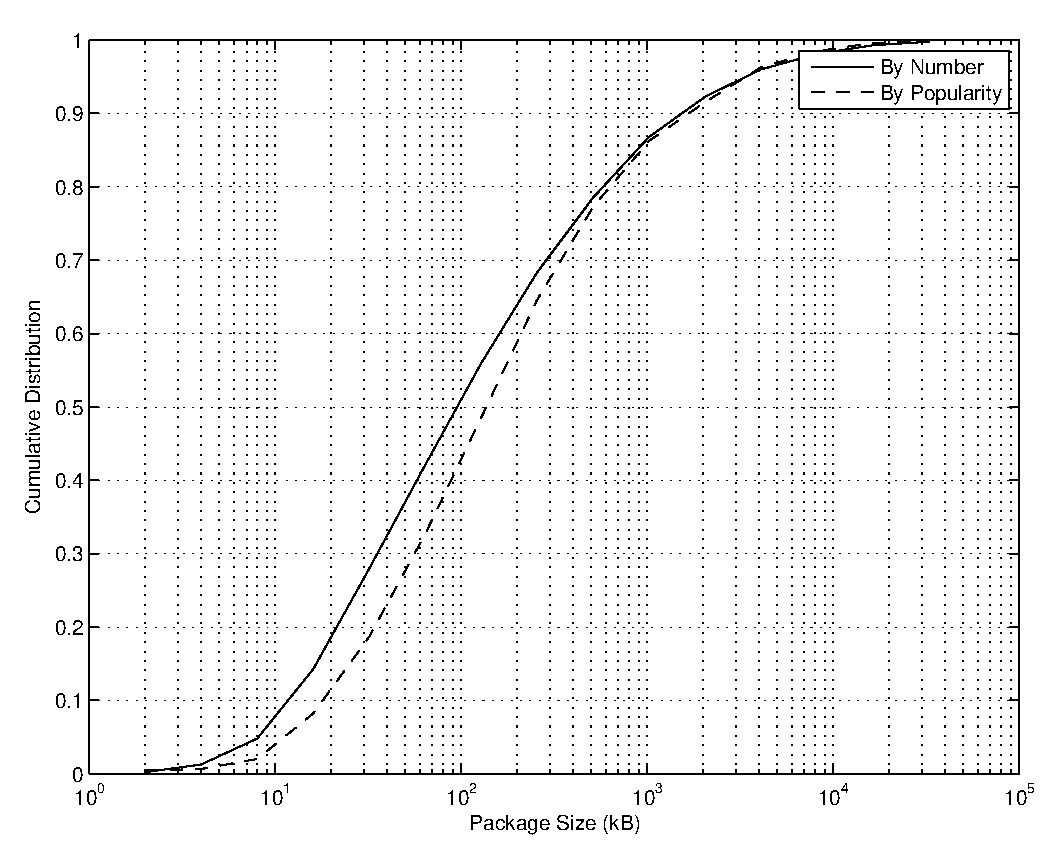
\includegraphics[width=\columnwidth]{apt_p2p_simulation-size_CDF.eps}
\caption{The CDF of the size of packages in a Debian system, both
for the actual size and adjusted size based on the popularity of
the package.}
\label{size_CDF}
\end{figure}

Figure \ref{size_CDF} shows the package size of the 22,298 packages
available in Debian in January 2008. We can see that most of the
packages are quite small, and so most will therefore not require
sub-piece information to download. We have chosen a piece
size of 512 kB, which means that 17,515 (78\%) of the packages will
not require this information. There are 3054 packages that will
require 2 to 4 pieces, for which the torrent string can be stored
directly with the package hash in the DHT. There are 1667 packages
that will require a separate lookup in the DHT for the longer
torrent string as they require 5 to 70 pieces. Finally, there are
only 62 packages that require more than 70 pieces, and so will
require a separate request to a peer for the torrent string.

\subsection{Current Status}
\label{status}

Though functional and useful, the current implementation is not
complete, and is missing some of the downloading details necessary.
It operates as a caching HTTP proxy, serving
requests from apt and other peers. Index files are identified by the
current implementation, and parsed to find the hashes of files for later DHT
lookups if they are requested. Files are downloaded from
peers, and those not available in peers are downloaded directly
from the mirror. Any downloaded files are hash checked to verify
them, and then added to the DHT.

However, the current implementation does not use the sub-piece
hashing described in section \ref{downloading}, or any parallelizing
of downloads. Instead, it currently chooses a peer at random from
the list of possible peers, and downloads the entire file from that
peer, regardless of the size of the file. This needs to change if
both a) the file is large (more than 512 KB), and b) there are
multiple peers with the file. The storage and retrieval of sub-piece
hashes has not yet been finalized though, and until it is this final
step is not possible.

%%%%%%%%%%%%%%%%%%%%%%%%%%%  Section  %%%%%%%%%%%%%%%%%%%%%%%%%%%%

\section{Future Work}
\label{future}

There are some additional steps to be taken to succeed with this
project. First, the storage method of sub-piece hashes needs to be
finalized and properly implemented. The communication built into the
Khashmir-based DHT also needs to be solidified. Some additional peer
statistics data needs to be made available for each peer, so that
some form of analysis is available once the system is deployed. The
reference implementation then needs to be packaged for upload to the
Debian package archive, so that it can benefit from the widest
possible deployment among users.

Finally, once deployed the system needs to be analyzed to determine
its effectiveness at meeting the goals of this project. The analysis
will consist of measuring, over time:
\begin{itemize}
 \item The number of peers using the system.
 \item The amount of downloaded data by peers from other peers.
 \item The amount of downloaded data by peers from mirrors/servers.
 \item The bandwidth used to maintain the DHT.
\end{itemize}

%%%%%%%%%%%%%%%%%%%%%%%%%%%  Section  %%%%%%%%%%%%%%%%%%%%%%%%%%%%

\section{Conclusions}
\label{conclusions}

We have designed a generally applicable peer-to-peer content
distribution model to be used by many of the free content
distributors operating today. It makes use of already existing
features of most package management systems, to create a
peer-to-peer distribution that should substantially reduce the costs
of hosting the content.

We have also implemented our design in software to be used in
conjuction with Debian-based distribution of Linux software
packages. It will soon be in use by many users of the Debian
project's distribution, and so serves as an example of the
possibilities that exist.

\bibliographystyle{IEEEtran}
\bibliography{./IEEEabrv,./all}

\end{document}
